\documentclass[11pt]{article}
\usepackage[margin=1in]{geometry}
\usepackage{amsmath,amssymb,bm}
\usepackage{tikz}
\usetikzlibrary{calc,arrows.meta}
\usepackage{algorithm}
\usepackage{algpseudocode}
\usepackage{booktabs}
\usepackage[hidelinks]{hyperref}

\newcommand{\T}{\bm{T}}
\newcommand{\s}{\bm{s}}
\newcommand{\h}{\bm{h}}

\title{The adjoint of the eikonal equation on a triangle mesh\\[2pt]
\large the gradient of the kinematic data likelihood with respect to the rupture velocities and the hypocenter}
\author{AlTar kinematic model on triangulated faults (\texttt{altar.models.seismic.kinematicmesh})}
\date{October 2026}

\begin{document}
\maketitle

\section{What the adjoint computes}

The kinematic model maps the parameters to the data in a chain:
\[
(\s, \h) \;\xrightarrow{\text{eikonal}}\; \T \;\xrightarrow{\text{interpolation}}\; T^I
\;\xrightarrow{\text{source time functions}}\; M_b \;\xrightarrow{G}\; \bm{d},
\]
where $s_p = 1/v_p$ is the slowness of patch $p$ (the inverse of its rupture velocity), $\h$
the hypocenter, $\T$ the rupture arrival times at the $V$ vertices of a mesh refined from the
patches, $T^I$ their interpolation to the source points of each patch, and $M_b$ the slip of each
patch in each time window. The data log likelihood is
$L = -\tfrac12\,(\bm{d}_{\rm obs} - G M_b)^{T} C^{-1} (\bm{d}_{\rm obs} - G M_b) + \text{const}$.

Back-propagating through $G$, the source time functions and the (linear) interpolation is
straightforward and gives $\bar{\bm g} = \partial L / \partial \T$, one number per vertex. This note is
about the remaining step: turning $\bar{\bm g}$ into $\partial L / \partial \s$ and
$\partial L/\partial \h$, at a cost independent of the number of parameters.

\section{The discrete eikonal equation and its fixed point}

The rupture front obeys $|\nabla T| = s$ on the fault surface. On a triangle mesh, the arrival
time at a vertex $C$ is updated from each triangle $(A, B, C)$ it belongs to, with slowness $s$:
the ray reaches $C$ from a point $P(\lambda) = (1-\lambda) A + \lambda B$ of the opposite edge,
\begin{equation}
U(T_A, T_B, s) \;=\; \min_{\lambda\in[0,1]} \Big[\, (1-\lambda)\,T_A + \lambda\,T_B
\;+\; s\,\big|C - P(\lambda)\big| \,\Big],
\label{eq:update}
\end{equation}
the time at $P$, interpolated along the edge, plus the travel time from $P$ to $C$
(Fig.~\ref{fig:update}). The minimum is at an interior $\lambda^\ast$ (a two-point update), in
closed form, or at an end (a one-point update, $T_A + s|AC|$ or $T_B + s|BC|$).

\begin{figure}[h]
\centering
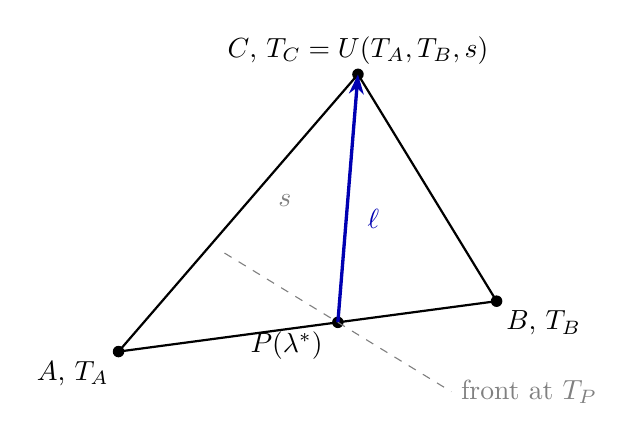
\begin{tikzpicture}[scale=1.6, >={Stealth[length=2.5mm]}]
  \coordinate (A) at (0,0); \coordinate (B) at (3,0.4); \coordinate (C) at (1.9,2.2);
  \coordinate (P) at ($(A)!0.58!(B)$);
  \draw[thick] (A) -- (B) -- (C) -- cycle;
  \fill (A) circle (1.3pt) node[below left] {$A$, $T_A$};
  \fill (B) circle (1.3pt) node[below right] {$B$, $T_B$};
  \fill (C) circle (1.3pt) node[above] {$C$, $T_C = U(T_A, T_B, s)$};
  \fill (P) circle (1.3pt) node[below left, xshift=-2pt] {$P(\lambda^\ast)$};
  \draw[->, very thick, blue!70!black] (P) -- (C);
  \node[blue!70!black, anchor=west] at (1.9,1.05) {$\ell$};
  \draw[dashed, gray] ($(P)+(-0.9,0.55)$) -- ($(P)+(0.9,-0.55)$) node[right, gray] {front at $T_P$};
  \node[gray] at (1.32,1.2) {$s$};
\end{tikzpicture}
\caption{The upwind update of $C$ from the edge $AB$ of a triangle of slowness $s$: the ray
crosses the edge at $P(\lambda^\ast)$ and travels $\ell = |C - P|$ to $C$.}
\label{fig:update}
\end{figure}

The arrival times are seeded with straight-ray times from the hypocenter near it,
$T^0_v(\h, s)$, and the fast iterative method (FIM) relaxes
$T_v \leftarrow \min\big(T_v,\, \min_{\text{triangles}} U\big)$ on the active vertices until nothing
changes. Its iterations depend on the data, but its \emph{fixed point} does not: at
convergence every vertex either keeps its seed or took its value from one winning triangle,
\begin{equation}
T_v = T^0_v(\h, s) \quad\text{(seeded)}, \qquad\text{or}\qquad
T_v = U\big(T_{a(v)},\, T_{b(v)},\, s_{p(v)}\big),
\label{eq:fixedpoint}
\end{equation}
with $a(v), b(v)$ its two \emph{parents} and $p(v)$ the patch of the winning triangle. We
differentiate~\eqref{eq:fixedpoint}, not the iterations.

\section{The local derivatives: the envelope theorem}

Write $f(\lambda) = (1-\lambda)T_A + \lambda T_B + s\,|C-P(\lambda)|$, so that $U = f(\lambda^\ast)$.
At an interior minimum $\partial f/\partial\lambda = 0$, so the dependence of $\lambda^\ast$ on
$(T_A, T_B, s)$ drops out (at an end, $\lambda^\ast$ is fixed):
\begin{equation}
\frac{\partial U}{\partial T_A} = 1 - \lambda^\ast, \qquad
\frac{\partial U}{\partial T_B} = \lambda^\ast, \qquad
\frac{\partial U}{\partial s} = \ell = |C - P(\lambda^\ast)|.
\label{eq:local}
\end{equation}
The sensitivities to the upwind times are the interpolation weights of the crossing point, and the
sensitivity to the slowness is the length of the ray segment inside the triangle. Chained along a
ray back to the hypocenter, $\partial T_v/\partial s_p$ is the total length of the ray of $v$
inside patch $p$: the travel-time tomography kernel, here obtained without tracing any ray.

For a seed, $T^0_v = s\,\big(d + \kappa\,(\max(0, d - r))^2/\Delta\big)$, with
$d = |\bm{x}_v - \bm{X}(\h)|$, gives $\partial T^0_v/\partial s$ (the seed's path) and
$\partial T^0_v/\partial \h$ through the point $\bm{X}(\h)$ of the hypocenter on the fault and the
Jacobian of its patch's affine map.

\section{The chain rule is a triangular linear system}

Linearizing~\eqref{eq:fixedpoint} at the fixed point:
\begin{equation}
d\T = W\, d\T + B\, d\s + S\, d\h ,
\label{eq:linear}
\end{equation}
where row $v$ of $W$ holds $1-\lambda^\ast$ and $\lambda^\ast$ at the columns of its parents (zero for
a seed), $B$ the ray lengths $\ell$ at the column of its patch, and $S$ the seed derivatives.
On acute and right triangles the update is causal: it exceeds the times of both of its parents,
so a parent arrives strictly earlier than its child (this is the condition the caveats return to).
With the vertices ordered by arrival time $W$ is then strictly lower triangular and $I - W$ is
invertible:
\[
d\T = (I - W)^{-1}\,(B\, d\s + S\, d\h),
\qquad
\frac{\partial L}{\partial \s} = B^{T} \bm\mu, \quad
\frac{\partial L}{\partial \h} = S^{T} \bm\mu, \quad
\bm\mu = \bar{\bm g} + W^{T} \bm\mu .
\]
The adjoint variable $\bm\mu$ solves an upper triangular system: back substitution, the vertices
\emph{latest first}. When vertex $v$ is visited, every vertex that depends on it arrived later and
has already added its share to $\mu_v$, so $\mu_v$ is final and can be pushed to its own parents.

\begin{algorithm}[h]
\caption{The backward pass, for one sample}
\begin{algorithmic}[1]
\State $\bm\mu \gets \bar{\bm g}$;\; $\bm g_s \gets 0$;\; $\bm g_h \gets 0$
\For{$v$ in the vertices by decreasing $T_v$}
  \If{$v$ is seeded}
     \State $\bm g_h \mathrel{+}= \mu_v\, \partial T^0_v/\partial\h$;\quad
            $g_{s,\,\text{owner}(v)} \mathrel{+}= \mu_v\, \partial T^0_v/\partial s$
  \Else
     \State $\mu_{a(v)} \mathrel{+}= (1-\lambda^\ast_v)\,\mu_v$;\quad
            $\mu_{b(v)} \mathrel{+}= \lambda^\ast_v\,\mu_v$;\quad
            $g_{s,\,p(v)} \mathrel{+}= \ell_v\,\mu_v$
  \EndIf
\EndFor
\State $\partial L/\partial v_p = -s_p^2\, g_{s,p}$, summed over the patches of a velocity group if they share one
\end{algorithmic}
\end{algorithm}

This is the exact gradient of the discrete forward model, which is why it agrees with central
differences to $10^{-8}$--$10^{-9}$\, (relative). It is the discrete counterpart of the
adjoint-state method for first-arrival travel times (Leung \& Qian 2006; Taillandier et al.\ 2009),
in which the adjoint satisfies a transport equation integrated backward along the characteristics.

\section{A one-dimensional example, and what it says about rupture velocity}

Take a chain $T_1 = T_0 + s_1 d$, $T_2 = T_1 + s_2 d$ and $L = g_1 T_1 + g_2 T_2$. The backward
pass gives $\mu_2 = g_2$, then $\mu_1 = g_1 + \mu_2$, so
\[
\frac{\partial L}{\partial s_2} = g_2\, d, \qquad \frac{\partial L}{\partial s_1} = (g_1 + g_2)\, d .
\]
A patch's slowness collects the sensitivities of everything downstream of it. The data constrain
the arrival times; a patch's velocity enters only through the arrival times of the patches beyond
it, so velocities of patches along the same rupture paths trade off. In the synthetic tests the
posterior onset times were recovered to $\sim0.4$ s while per-patch velocities stayed loose, and a
coarser velocity parameterization (velocity groups) was resolved almost entirely.

\section{Implementation on the GPU}

In \texttt{cudaKinematicMesh}, for a batch of samples (chains):
\begin{enumerate}
\item \textbf{Parents}, one thread per (sample, vertex): recompute the winning update at the
converged $\T$, and store $a(v), b(v), p(v)$ and the three weights $(1-\lambda^\ast, \lambda^\ast, \ell)$,
or, for a seed, $\partial T^0_v/\partial\h$ and $\partial T^0_v/\partial s$.
\item \textbf{Order}: a segmented sort of the vertices of each sample by decreasing $T$
(CUB \texttt{DeviceSegmentedSort}).
\item \textbf{Backward pass}: one thread per sample walks that order, a few memory operations per
vertex; velocity gradients accumulate into shared columns for velocity groups.
\end{enumerate}
Memory: a few numbers per vertex and sample, against the snapshots of every sweep that the
adjoint of the structured fast-sweeping model keeps. Cost on the 96-patch synthetic (4941 vertices,
4096 chains, float32): the forward model takes about 45 ms, the adjoint adds about 15 ms.

\begin{table}[h]
\centering
\begin{tabular}{lr}
\toprule
check (\texttt{models/seismic/tests/kinematic\_mesh.py}) & relative difference \\
\midrule
$M_b$, CUDA against the NumPy prototype & $8\times10^{-16}$ \\
gradient, CUDA against the prototype & $3\times10^{-15}$ \\
gradient against central differences & $2\times10^{-9}$ \\
grouped velocities, against central differences & $1\times10^{-9}$ \\
\bottomrule
\end{tabular}
\end{table}

\section{Caveats}

\begin{itemize}
\item \textbf{Kinks.} $\T$ is piecewise smooth: where two candidate updates tie, where two rupture
fronts meet, or where a seed and an update tie, the gradient jumps. These sets have measure zero
and have not troubled HMC.
\item \textbf{Ordering.} The backward pass assumes each parent arrived strictly earlier; it holds on
acute and right triangles (the prototype counts violations and found none). Obtuse triangles can
break causality and should be avoided or split in real slab meshes.
\item \textbf{Convergence.} The parents must be those of the converged solution; FIM is run to an
exact fixed point (no tolerance).
\end{itemize}

\section*{References}
\small
\begin{itemize}
\item Jeong, W.-K., Whitaker, R.\,T. (2008). A fast iterative method for eikonal equations.
\emph{SIAM J. Sci. Comput.} 30, 2512--2534.
\item Fu, Z., Jeong, W.-K., Pan, Y., Kirby, R.\,M., Whitaker, R.\,T. (2011). A fast iterative method
for solving the eikonal equation on triangulated surfaces. \emph{SIAM J. Sci. Comput.} 33,
2468--2488.
\item Leung, S., Qian, J. (2006). An adjoint state method for three-dimensional transmission
traveltime tomography using first-arrivals. \emph{Commun. Math. Sci.} 4, 249--266.
\item Taillandier, C., Noble, M., Chauris, H., Calandra, H. (2009). First-arrival traveltime
tomography based on the adjoint-state method. \emph{Geophysics} 74, WCB1--WCB10.
\item Minson, S.\,E., Simons, M., Beck, J.\,L. (2013). Bayesian inversion for finite fault earthquake
source models I. \emph{Geophys. J. Int.} 194, 1701--1726.
\end{itemize}

\end{document}
